

\subsection{Disjoint Cycle Packing}
In this subsection we  design a PSAKS for the {\sc Disjoint Cycle Packing ($CP$)} problem. 
The parameterized optimization problem {\sc Disjoint Cycle Packing ($CP$)} is formally defined as,
\[
    CP(G,k,P)=\left\{ 
\begin{array}{rl}
    -\infty & \text{if $P$ is not a set of vertex disjoint cycles in $G$} \\
    \min\left\{|P|,k+1\right\} & \text{otherwise}
\end{array}\right.
\]




We start by defining feedback vertex sets of a graph. Given a graph $G$ and a vertex subset $F\subseteq V(G)$, $F$ is called a {\em feedback veretx set} of $G$ if $G-F$ is a forest. 
We will make use of the following well-known Erd\H{o}s-P\'{o}sa Theorem relating feedback vertex set and the number of vertex disjoint  cycles in a graph. 
\begin{lemma}[\cite{ErdosPosa1965}]
\label{lemma:erdosposa}
There exists a constant $c$ such that for each positive integer $k$, every (multi) graph either contains $k$ vertex disjoint cycles or it has a feedback vertex set of size at most $ck\log k$. Moreover, there is a polynomial time algorithm that takes a graph $G$ and an integer $k$ as input, and outputs either $k$ vertex disjoint cycles or a feedback vertex set of size at most $ck\log k$. 
\end{lemma}

 The following lemma allows us to reduce the size of the input 
graph $G$ if it has a small feedback vertex set. 

\begin{lemma}
 \label{lemma:leaf}
 Let $(G,k)$ be an instance of \CP{} and $F$ be a feedback vertex set of $G$. Suppose there are strictly  
 more than $\vert F\vert^2(2\vert F\vert+1)$ vertices in $G-F$ whose degree in $G-F$ is at most $1$. 
Then there is a polynomial time 
algorithm ${\cal A}$ that, given an instance $(G,k)$ and a feedback vertex set satisfying the above properties,
  returns a graph $G'$ (which is a minor of $G$) such that $OPT(G,k)=OPT(G',k)$, $\vert V(G')\vert =\vert V(G)\vert -1$ and $F \subseteq V(G')$ is still a feedback vertex set of $G'$.  
Further, given a cycle packing ${\cal S'}$ in $G'$, there is a polynomial time algorithm ${\cal B}$ which 
outputs a cycle packing ${\cal S}$ in $G$ such that $\vert {\cal S}\vert=\vert {\cal S'}\vert$. 
\end{lemma}


\begin{proof}
The algorithm ${\cal A}$ works as follows. 
 Let $|F|=\ell$ and  for $(u,v)\in F\times F$, let $L(u,v)$ be the set of vertices of degree at most $1$ in $G-F$ such that each $x\in L(u,v)$ is adjacent to both $u$ and $v$ (if $u=v$, then $L(u,u)$
is the set of vertices which have degree at most $1$ in $G-F$ and at least two edges to $u$). Suppose that the number of vertices of degree at most $1$ in $G-F$ is strictly more than
$\ell^2(2\ell+1)$. For each pair $(u,v)\in F\times F$, if $L(u,v)>2\ell+1$ then we mark an arbitrary  set of 
$2\ell+1$ vertices from $L(u,v)$, else we mark all the vertices in $L(u,v)$. Since there are at most $\ell^2(2\ell+1)$ marked vertices,
there exists an unmarked vertex $w$ in $G-F$ such that 
 $d_{G-F}(w)\leq 1$. 
If $d_{G-F}(w)=0$, then algorithm ${\cal A}$
returns $(G-w,k)$.
Suppose $d_{G-F}(w)=1$. Let  $e$ be the unique edge in $G-F$ which is incident to $w$. Algorithm ${\cal A}$  
returns $(G/e,k)$. Clearly $F\subseteq V(G')$ and $F$ is a feedback vertex set of $G'$. 

 Let $(G',k)$ be the instance returned by algorithm ${\cal A}$.
Since $G'$ is a minor of $G$, $OPT(G,k)\geq OPT(G',k)$.   (A graph $H$ is called a minor of an undirected  graph $G^\star$, if we  can obtain $H$ from $G^\star$ by a sequence of edge deletions, vertex deletions and edge contractions.) 
Now we show that $OPT(G,k)\leq OPT(G',k)$. 
Let $G'=G/e$, $e=(w,z)$, $d_{G-F}(w)=1$ and $w$ is an unmarked vertex.   
 Let $\CC$ be a maximum set of vertex disjoint cycles in $G$. Observe that if $\CC$ does not contain a pair of cycles each intersecting a different endpoint of $e$, then contracting $e$ will keep the resulting cycles vertex disjoint in $G/e$. Therefore, we may assume that $\CC$ contains 2 cycles $C_w$ and $C_z$ where $C_w$ contains $w$ and $C_z$ contains $z$. Now, the neighbor(s) of $w$ in $C_w$ must lie in $F$. Let these neighbors be $x$ and $y$ (again, $x$ and $y$ are not necessarily distinct). Since $w\in L(x,y)$ and it is unmarked, there are $2\ell+1$ vertices in $L(x,y)$ which are already marked by the marking procedure. 
Further, since for each vertex $u\in V(\CC)$, with $d_{G-F}(u)\leq 1$, 
at least one neighbour of $u$ in the cycle packing $\CC$ is from $F$  and each  
vertex  $v\in V(\CC)\cap F$ can be adjacent to at most $2$ vertices from 
$L(x,y)$, we have that at most $2\ell$ vertices from $L(x,y)$ are in $V(\CC)$. This implies that 
at least one vertex (call it $w'$), marked for $L(x,y)$ is not in   $V(\CC)$. 
Therefore we can route the cycle $C_w$ through $w'$ instead of $w$, which gives us a set of $\vert \CC\vert$ vertex disjoint cycles in $G/e$. 
Suppose $G'=G-w$ and $d_{G-F}(w)=0$. Then by similar arguments we can show that 
$OPT(G,k)=OPT(G-w,k)$. 

Algorithm ${\cal B}$ takes a solution ${\cal S'}$ of the instance $(G',k)$ and outputs a solution ${\cal S}$ of $(G,k)$ 
as follows. If $G'$ is a subgraph of $G$ (i.e, $G'$ is obtained by deleting a vertex), then ${\cal S}={\cal S'}$. Otherwise, 
let $G'=G/e$, $e=(u,v)$ and let $w$ be the vertex in $G'$ created by contracting $(u,v)$. If $w\notin V({\cal S}')$, then 
${\cal S}={\cal S}'$. Otherwise let $C=wv_1\ldots v_{\ell}$ be the cycle in ${\cal S}'$ containing $w$. 
We know that $v_1,v_\ell \in N_G(\{u,v\})$. 
If $v_1,v_{\ell}\in N_G(u)$, then $C'=uv_1\ldots v_{\ell}$ is a cycle in $G$ which is vertex disjoint 
from ${\cal S'}\setminus \{C\}$. If $v_1,v_{\ell}\in N_G(v)$,  then $C'=vv_1\ldots v_{\ell}$ is a cycle in $G$ which is vertex disjoint 
from ${\cal S'}\setminus \{C\}$. In either case ${\cal S}=({\cal S'}\setminus \{C\})\cup \{C'\}$. 
If $v_1\in N_G(u)$ and $v_{\ell}\in N_G(v)$, then $C''=uv_1\ldots v_\ell vu$ is 
a cycle in $G$ which is vertex disjoint 
from ${\cal S'}\setminus \{C\}$. In this case ${\cal S}=({\cal S'}\setminus \{C\})\cup \{C''\}$.
This completes the proof of the lemma.
\end{proof}



Lemma~\ref{lemma:leaf} leads to the following reduction rule which is \onesafe{} (follows from Lemma~\ref{lemma:leaf}). 

\begin{redrule}
\label{rule:leaf}
 Let $(G,k)$ be an instance of \CP{} and let $F$ be a feedback vertex set of $G$ 
such that the forest $G-F$ contains strictly  
 more than $\vert F\vert^2(2\vert F\vert+1)$ vertices of degree at most $1$.  
Then run the algorithm ${\cal A}$ mentioned in Lemma~\ref{lemma:leaf} 
on $(G,k)$ and $F$, and return $(G',k)$, where $G'$, a minor of $G$, is the output of the algorithm ${\cal A}$.   
\end{redrule}


The following observation follows from Lemma~\ref{lemma:leaf}. 
\begin{observation}
\label{obs:leaf_opt}
Let $(G,k)$ be an instance of \CP{} and $(G',k)$ be the instance obtained after applying  
Reduction Rule~\ref{rule:leaf}. Then $OPT(G,k)=OPT(G',k)$. 
\end{observation}

The Reduction Rule~\ref{rule:leaf}, may create multiple edges in the reduced instance.  
To bound the number of multi-edges between a pair of vertices, we use the following 
simple reduction rule. 
\begin{redrule}
 \label{rule:multiedge}
 Let $(G,k)$ be an instance of \CP{} and there exist two vertices $u,v\in G$ such that 
 there are at least $3$ edges between $u$ and $v$. Then delete all but two edges between $u$ and 
 $v$.  
\end{redrule} 

Since any set of vertex disjoint cycles in $G$ can use at most two edges between $u$ and $v$, 
it is safe to delete remaining edges between them and hence Reduction Rule~\ref{rule:multiedge} 
is \onesafe.  Hence, in the rest of the section we always assume that 
the number of edges between any pair of vertices is at most $2$. 
The following lemma allows us to find a subset $F'$, of a feedback vertex set $F$, of cardinality at most $OPT(G,k)$ such that the large portion of the graph $G-F$ is connected to $F'$ and not to $F\setminus F'$.  


\begin{figure}

 \begin{subfigure}[b]{0.5\textwidth}
        \centering

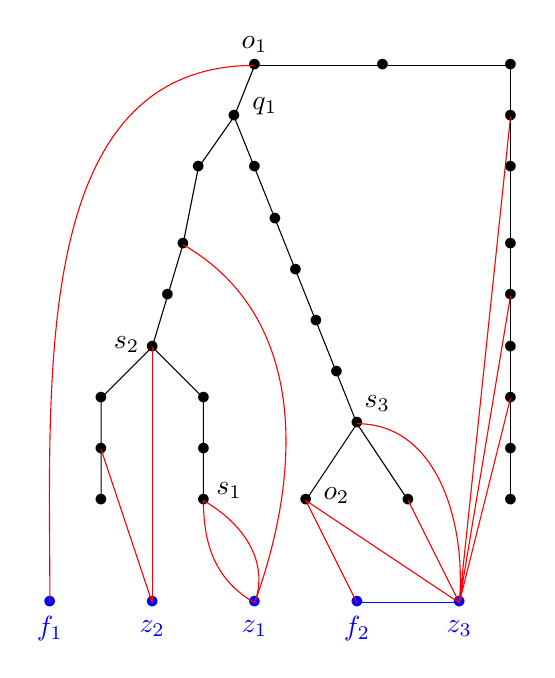
\begin{tikzpicture}[scale=1.3]


\node [] (a) at (0,0.75) {$\bullet$};
\node [] (a) at (1,0.75) {$\bullet$};
\node [] (a) at (2,0.75) {$\bullet$};
\node [] (a) at (2.3,0.8) {$o_2$};
\node [] (a) at (3,0.75) {$\bullet$};
\node [] (a) at (4,0.75) {$\bullet$};
\node [] (a) at (1.25,0.85) {$s_1$};


\node [] (a) at (0,1.25) {$\bullet$};
\node [] (a) at (1,1.25) {$\bullet$};
\node [] (a) at (0,1.75) {$\bullet$};
\node [] (a) at (1,1.75) {$\bullet$};
\node [] (a) at (0.5,2.25) {$\bullet$};
\node [] (a) at (0.25,2.27) {$s_2$};
\node [] (a) at (0.65,2.75) {$\bullet$};
\node [] (a) at (0.8,3.25) {$\bullet$};
\node [] (a) at (0.95,4) {$\bullet$};
\node [] (a) at (1.5,5) {$\bullet$};
\node [] (a) at (1.5,5.2) {$o_1$};


\draw (0,0.75)--
 (0,1.25) --
(0,1.75)  -- 
(0.5,2.25) -- (0.65,2.75) -- (0.8,3.25)--  (0.95,4) -- (1.3,4.5)--(1.5,5);
\draw (1,0.75) --
(1,1.25) -- (1,1.75)--(0.5,2.25);




\node [] (a) at (2.5,1.5) {$\bullet$};
\node [] (a) at (2.7,1.7) {$s_3$};
\node [] (a) at (2.3,2) {$\bullet$};

\node [] (a) at (2.1,2.5) {$\bullet$};
\node [] (a) at (1.9,3) {$\bullet$};
\node [] (a) at (1.7,3.5) {$\bullet$};
\node [] (a) at (1.5,4) {$\bullet$};
\node [] (a) at (1.3,4.5) {$\bullet$};
\node [] (a) at (1.6,4.6) {$q_1$};


\draw (2,0.75)--
(2.5,1.5) --(2.3,2) --
(2.1,2.5)--(1.9,3) -- (1.7,3.5) -- (1.5,4) -- (1.3,4.5);
\draw (3,0.75)--(2.5,1.5);



\node [] (a) at (4,1.25) {$\bullet$};
\node [] (a) at (4,1.75) {$\bullet$};
\node [] (a) at (4,2.25) {$\bullet$};
\node [] (a) at (4,2.75) {$\bullet$};
\node [] (a) at (4,3.25) {$\bullet$};
\node [] (a) at (4,4) {$\bullet$};
\node [] (a) at (4,4.5) {$\bullet$};
\node [] (a) at (4,5) {$\bullet$};

\node [] (a) at (2.75,5) {$\bullet$};


\draw (4,0.75)--
 (4,1.25) --(4,1.75) -- (4,2.25) -- (4,2.75) -- (4,3.25) -- (4,4) -- (4,4.5) -- (4,5)-- (2.75,5)  --  (1.5,5);



\node [blue] (a) at (-0.5,-0.25) {$\bullet$};
\node [blue] (a) at (0.5,-0.25) {$\bullet$};
\node [blue] (a) at (1.5,-0.25) {$\bullet$};
\node [blue] (a) at (2.5,-0.25) {$\bullet$};
\node [blue] (a) at (3.5,-0.25) {$\bullet$};

\node [blue] (a) at (-0.5,-0.5) {$f_1$};
\node [blue] (a) at (0.5,-0.5) {$z_2$};
\node [blue] (a) at (1.5,-0.5) {$z_1$};
\node [blue] (a) at (2.5,-0.5) {$f_2$};
\node [blue] (a) at (3.5,-0.5) {$z_3$};


\draw[blue] (2.5,-0.25) -- (3.5,-0.25);

\draw[red] (1.5,-0.25) to [out=150,in=270] (1,0.75);
\draw[red] (1.5,-0.25) to [out=70,in=-30] (1,0.75);
\draw[red] (3.5,-0.25) -- (4,1.75)
 (3.5,-0.25) -- (4,2.75) 
(3.5,-0.25) -- (4,4.5);
\draw[red] (1.5,-0.25) to [out=70,in=-30] (0.8,3.25);

\draw[red] 
(3.5,-0.25) --(2,0.75) 
 (3.5,-0.25) -- (3,0.75) 
 (3.5,-0.25) to [out=85,in=0] (2.5,1.5);  



\draw[red] (2,0.75) -- (2.5,-0.25);


\draw[red] (0.5,-0.25) -- (0,1.25);
\draw[red] (0.5,2.25)-- (0.5,-0.25);

\draw[red] (-0.5,-0.25)  to [out=90,in=180]  (1.5,5);

\end{tikzpicture}
\caption{$F=\{f_1,f_2,z_1,z_2,z_3\}$ is a feedback vertex set of $G$ and the tree $G-F$ is rooted 
at $o_1$. Algorithm ${\cal B}$ will output $F'=\{z_1,z_2,z_3\}$ and 
$S=\{s_1,s_2,s_3\}$ when $k>3$.} 
\label{fig:atreemarking}
\end{subfigure}
\begin{subfigure}[b]{0.5\textwidth}
        \centering

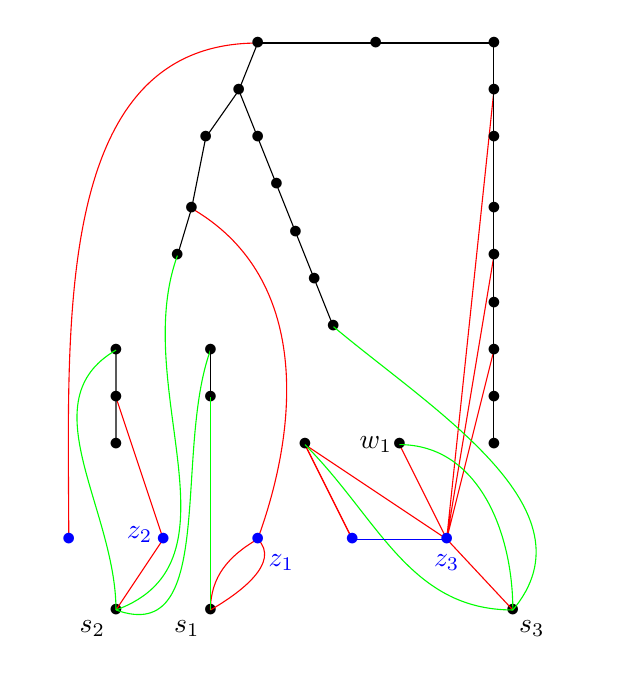
\begin{tikzpicture}[scale=1.2]




\node [] (a) at (-0.25,-1.2) {$s_2$};
\node [] (a) at (0,-1) {$\bullet$};
\node [] (a) at (1,-1) {$\bullet$};
\node [] (a) at (0.75,-1.2) {$s_1$};
\node [] (a) at (4.2,-1) {$\bullet$};
\node [] (a) at (4.4,-1.2) {$s_3$};



\draw[red] (1.5,-0.25) to [out=210,in=90] (1,-1);
\draw[red] (1.5,-0.25) to [out=-45,in=30] (1,-1);

\draw[red] (3.5,-0.25) -- (4,1.75)
 (3.5,-0.25) -- (4,2.75) 
(3.5,-0.25) -- (4,4.5);
\draw[red] (1.5,-0.25) to [out=70,in=-30] (0.8,3.25);

\draw[red] (3.5,-0.25) --(2,0.75) 
 (3.5,-0.25) -- (3,0.75) 
 (3.5,-0.25)--(4.2,-1);


\draw[red] (2,0.75) -- (2.5,-0.25);

\draw[red] (2,0.75) -- (2.5,-0.25);


\draw[red]  (0,-1) -- (0.5,-0.25);
\draw[red] (0,1.25)-- (0.5,-0.25);


\draw[red] (-0.5,-0.25)  to [out=90,in=180]  (1.5,5);



\node [] (a) at (0,0.75) {$\bullet$};
\node [] (a) at (2,0.75) {$\bullet$};
\node [] (a) at (3,0.75) {$\bullet$};
\node [] (a) at (4,0.75) {$\bullet$};
\node [] (a) at (2.75,0.75) {$w_1$};


\node [] (a) at (0,1.25) {$\bullet$};
\node [] (a) at (1,1.25) {$\bullet$};
\node [] (a) at (0,1.75) {$\bullet$};
\node [] (a) at (1,1.75) {$\bullet$};
\node [] (a) at (0.65,2.75) {$\bullet$};
\node [] (a) at (0.8,3.25) {$\bullet$};
\node [] (a) at (0.95,4) {$\bullet$};
\node [] (a) at (1.5,5) {$\bullet$};

\draw (0,0.75)-- (0,1.25)
 --(0,1.75)
(0.65,2.75) -- 
(0.8,3.25)--  
(0.95,4) -- (1.3,4.5)--(1.5,5);
\draw[green]
(0,1.75) to [out=210,in=90] (0,-1)
(1,1.75) to [out=250,in=-20] (0,-1)
(0.65,2.75) to [out=250,in=20] (0,-1);

\draw [green]
(1,-1)--
(1,1.25);
\draw (1,1.25)
 -- (1,1.75);





\node [] (a) at (2.3,2) {$\bullet$};

\node [] (a) at (2.1,2.5) {$\bullet$};
\node [] (a) at (1.9,3) {$\bullet$};
\node [] (a) at (1.7,3.5) {$\bullet$};
\node [] (a) at (1.5,4) {$\bullet$};
\node [] (a) at (1.3,4.5) {$\bullet$};

\draw[green] (2,0.75) to [out=-45,in=180]
(4.2,-1) to [out=50,in=-40] (2.3,2);
\draw
(2.3,2) --
(2.1,2.5)--(1.9,3) -- (1.7,3.5) -- (1.5,4) -- (1.3,4.5);
\draw[green] (3,0.75)  to [out=0,in=90] (4.2,-1);




\node [] (a) at (4,1.25) {$\bullet$};
\node [] (a) at (4,1.75) {$\bullet$};
\node [] (a) at (4,2.25) {$\bullet$};
\node [] (a) at (4,2.75) {$\bullet$};
\node [] (a) at (4,3.25) {$\bullet$};
\node [] (a) at (4,4) {$\bullet$};
\node [] (a) at (4,4.5) {$\bullet$};
\node [] (a) at (4,5) {$\bullet$};

\node [] (a) at (2.75,5) {$\bullet$};


\draw (4,0.75)--
 (4,1.25) --(4,1.75) -- (4,2.25) -- (4,2.75) -- (4,3.25) -- (4,4) -- (4,4.5) -- (4,5)-- (2.75,5)-- (1.5,5);



\node [blue] (a) at (-0.5,-0.25) {$\bullet$};
\node [blue] (a) at (0.5,-0.25) {$\bullet$};
\node [blue] (a) at (1.5,-0.25) {$\bullet$};
\node [blue] (a) at (2.5,-0.25) {$\bullet$};
\node [blue] (a) at (3.5,-0.25) {$\bullet$};

\node [blue] (a) at (0.25,-0.2) {$z_2$};
\node [blue] (a) at (1.75,-0.5) {$z_1$};
\node [blue] (a) at (3.5,-0.5) {$z_3$};


\draw[blue] (2.5,-0.25) -- (3.5,-0.25);



\end{tikzpicture}
\caption{The vertices of $S$ is drawn separately with edges between $S$ and $G-F$ colored green}
\label{fig:btreemarking}
\end{subfigure}

\caption{An example of Lemma~\ref{lemma:mark_in_tree}}
\label{fig:treemarking}
\end{figure}
 

\begin{lemma}
\label{lemma:mark_in_tree}
Let $(G,k)$ be an instance of \CP{} and let $F$ be a feedback vertex set of $G$. Then there is 
a polynomial time algorithm ${\cal B}$ that given $(G,k)$ and $F$, either outputs $k$ 
vertex disjoint cycles in $G$ or two sets $F'\subseteq F$ and $S\subseteq V(G-F)$ such that 
$(i)$ $\vert F'\vert, \vert S\vert \leq OPT(G,k)$ and $(ii)$ for any $w\in F \setminus F'$ and any connected component $C$ of $G-(F\cup S)$, 
$\vert N(w)\cap V(C)\vert \leq 1$. 
\end{lemma}
\begin{proof}
We know that $G-F$ is a forest. We consider each tree in $G-F$ as a rooted tree, where the root is chosen arbitrarily. Now we create a 
{\em dummy root $r$} and connect to all the roots in $G-F$. The resulting graph $T$ with vertex set $(V(G)\cup \{r\})\setminus F$ is 
a tree rooted at $r$. The level of a vertex $v\in V(T)$ is the distance between $r$ and $v$, denoted by $d_T(r,v)$. Let $T'$ be a rooted tree, then for a vertex $v\in V(T')$  
we use $T'_v$ to denote the subtree of $T'$ rooted at $v$.  

Now we are ready to give a procedure to find the desired sets 
$F'$ and $S$. Initially we set $T':=T$, $F':=\emptyset$ and $S:=\emptyset$. Let $u\in V(T')$ such that 
$d_{T'}(r,u)$ is maximized and there is a vertex $w\in F\setminus F'$ with the property that $G[V(T'_u)\cup \{w\}]$ has a cycle.  
Then, we set $T':=T'-T'_u$, $F':=F'\cup\{w\}$ and $S:=S\cup \{u\}$. We continue this procedure until $\vert F'\vert=\vert S \vert=k$ 
or the above step is not applicable. Let $F'=\{w_1,\ldots,w_{k'}\}$.
Notice that by the above process there are vertex disjoint subtrees 
$T_1,\ldots,T_{k'}$ of $T-r$  such that for each $i\in [k']$, $G[V(T_i)\cup \{w_i\}]$ has a cycle. 
Thus when $k'=k$, our algorithm 
${\cal B}$ will output one cycle from each $G[V(T_i)\cup \{w_i\}]$, $i\in [k]$ as the output. Otherwise, since in each step the 
algorithm picks a vertex with highest level, each connected component $C$ of $T-S$ and $w\in F \setminus F'$,  
$\vert N(w)\cap V(C)\vert \leq 1$. 
Algorithm ${\cal B}$ will output 
$F'$ and $S$ are the required sets. Notice that, in this case $\vert F'\vert=\vert S \vert =k'<k$. We have seen that there are $\vert F'\vert$ vertex disjoint cycles in $G$. This implies that   $\vert F'\vert=\vert S \vert \leq OPT(G,k)$.  An illustration is given in Figure~\ref{fig:treemarking}.  Figure~\ref{fig:atreemarking} depicts a graph $G$ with a feedback vertex set $F$ and 
the sets $F'$ and $S$ chosen by the algorithm. In Figure~\ref{fig:btreemarking}, the graph $G-(F'\cup S)$ is drawn separately 
to see the properties mentioned in the lemma.  
 
\end{proof}

Using Lemma~\ref{lemma:mark_in_tree}, we will prove the following decomposition lemma and after this the structure of the reduced graph becomes ``nice'' and our algorithm boils down to applications of \shortULI{$\epsilon$} on multiple auxiliary interval graphs.  


\begin{lemma}
\label{lem:CP_path_creation}
Let $(G,k)$ be an instance of \CP. Then there is a polynomial time algorithm ${\cal A}$ which either 
outputs $k$ vertex disjoint cycles or 
a minor $G'$ of $G$, and $Z,R\subseteq V(G')$ with the following properties.
\begin{itemize}
\setlength{\itemsep}{-2pt}
\item[$(i)$] $OPT(G,k)=OPT(G',k)$, 
\item[$(ii)$] $\vert Z \vert \leq OPT(G,k)$, $\vert R\vert = \OO(k^4\log^4 k)$, 
\item[$(iii)$] $G'-(Z\cup R)$ is a  collection $\cP$ of  $\OO(k^4\log^4 k)$ non trivial paths, and 
\item[$(iv)$] for each path $P=u_1\cdots u_r$ in $\cP$, no internal vertex is adjacent to a vertex in $R$, \;
$d_{G'[R\cup \{u_1\}]}(u_1)  \leq 1$, and $d_{G'[R\cup \{u_r\}]}(u_r) \leq 1$.
\end{itemize}
Furthermore, given a cycle packing ${\cal S'}$ in $G'$, there is a polynomial time algorithm ${\cal D}$ which 
outputs a cycle packing ${\cal S}$ in $G$ such that $\vert {\cal S}\vert=\vert {\cal S'}\vert$. 
\end{lemma}

\begin{proof}
We first give a description of the polynomial time algorithm ${\cal A}$ mentioned in the statement of the lemma. 
It starts by running  the algorithm mentioned in Lemma~\ref{lemma:erdosposa} on input $(G,k)$ and if it returns $k$ vertex disjoint cycles,  then ${\cal A}$ returns 
$k$ vertex disjoint cycles in $G$ 
and stops. Otherwise, let $F$ be a 
feedback vertex set of $G$. 
Now  ${\cal A}$ applies Reduction Rule~\ref{rule:leaf} repeatedly using the feedback vertex set $F$ until 
Reduction Rule~\ref{rule:leaf} is no longer applicable. Let $(G',k)$ be the reduced instance after the exhaustive application of 
Reduction Rule~\ref{rule:leaf}. By Lemma~\ref{lemma:leaf}, we have that $F\subseteq V(G')$ and $G'-F$ is a forest. 
Now,  ${\cal A}$ runs the algorithm ${\cal B}$ mentioned in Lemma~\ref{lemma:mark_in_tree} on input $(G',k)$ and $F$. If ${\cal B}$ 
returns $k$ vertex disjoint cycles in $G'$, then ${\cal A}$ also returns $k$ vertex disjoint cycles in $G$. The last assertion follows from the fact that  Reduction Rule~\ref{rule:leaf} (applied to get $G'$) is \onesafe. 
Otherwise, let $F'\subseteq F$ and $S\subseteq V(G'-F)$ be the output of ${\cal B}$. Next we define a 
few sets that will be used by $\cal A$ to construct its output.
\begin{enumerate}
\setlength{\itemsep}{-2pt}
\item Let $Q$ be the set 
of vertices of $G'-F$ whose  degree in $G'-F$ is at least $3$. 
\item Let $O=\bigcup_{w\in F\setminus F'} N(w)\cap V(G'-F)$; and 
\item let $W$ be the vertices of degree $0$ in $G'-(F\cup Q\cup O \cup S)$. 
\end{enumerate}
Algorithm ${\cal A}$ returns $G'$, $Z=F'$ and 
$R=Q\cup O \cup S\cup W \cup (F\setminus F')$ as output. In the example given in Figure~\ref{fig:treemarking}, $Z=\{z_1,z_2,z_3\}, F\setminus F'=\{f_1,f_2\}, S=\{s_1,s_2,s_3\}, Q=\{q_1,s_2,s_3\}, O=\{o_1,o_2\}$ and $W=\{w_1\}$.

Now we prove the correctness of the algorithm. If ${\cal A}$ outputs $k$ vertex disjoint  cycles in $G$, then we are done. Otherwise, let $Z=F'$ and $R=Q\cup O \cup S\cup W \cup (F\setminus F')$ be the output of ${\cal A}$. 
Now we prove $G', Z$ and $R$  indeed satisfy the properties mentioned in the statement of lemma.
Since $G'$ is obtained after repeated applications of Reduction Rule~\ref{rule:leaf}, by Observation~\ref{obs:leaf_opt}, we get 
that $OPT(G,k)=OPT(G',k)$ and hence proving property $(i)$.  


By Lemma~\ref{lemma:mark_in_tree}, 
we have that $\vert F'\vert= \vert S \vert \leq OPT(G,k)$. Hence the size of $Z(=F')$ is as desired. 
Next we bound the size of $R$.  
By  Lemma~\ref{lemma:erdosposa}, we have that $\vert F\vert\leq ck\log k$, where $c$ is a fixed constant.   
By Lemma~\ref{lemma:leaf}, we have that $F\subseteq V(G')$, $G'-F$ is a forest, and 
the number of vertices of  degree at most $1$ in $G'-F$ is upper bounded by $\vert F\vert^2(2\vert F\vert+1)=\OO(k^3\log^3 k)$. 
Since the number of vertices of degree at least $3$ in a forest is at most the number of leaves in the forest, we can conclude 
that cardinality of $Q$, the set of vertices of degree at least $3$ in $G'-F$ is upper bounded by $\OO(k^3\log^3 k)$. It is well-known that the number of maximal degree $2$ paths in a forest is  upper bounded by the sum of the number of leaves and the vertices of degree at least $3$ 
(for example see~\cite{RamanSS06} for a proof). This immediately implies the following claim. 

\begin{claim}
 \label{claim:no_of_paths}
 $G'-(F\cup Q)$ is a collection of $\OO(k^3\log^3 k)$ paths. 
\end{claim}
The following claim proves properties $(ii)$ and $(iii)$ stated in the lemma. 
\begin{claim}
\label{claim:CPboundR}
$\vert R\vert = \OO(k^4\log^4 k)$ and the number of paths in $\cP$ is at most  $\OO(k^4\log^4 k)$. 
\end{claim}
\begin{proof}
Observe that $G'-(F\cup Q)$ is a 
collection of $\OO(k^3\log^3 k)$ paths and thus it has at most  $\OO(k^3\log^3 k)$ connected components. This implies that, $G'-(F\cup Q \cup S)$ has at most  $\OO(k^3\log^3 k)$ connected components and in particular $G'-(F \cup S)$ has at most  $\OO(k^3\log^3 k)$ connected components. 
Let $\gamma_s$ denote the number of connected components of $G'-(F \cup S)$. 
By Lemma~\ref{lemma:mark_in_tree}, we have that 
for any $w\in F \setminus F'$ and any connected component $C$ of $G'-(F\cup S)$, 
$\vert N_{G'}(w)\cap V(C) \vert \leq 1$.  Thus, for every vertex  $w\in F \setminus F'$ we have that 
$|N(w)\cap V(G'-F)|\leq |S|+ \gamma_s=\OO(k^3\log^3 k)$. 
This
implies that the cardinality of $O$, the set $\bigcup_{w\in F\setminus F'} N(w)\cap V(G'-F)$,  
is upper bounded by $\OO( \vert F \setminus F'\vert \cdot k^3\log^3 k)=\OO( k^4\log^4 k)$.  
By Lemma~\ref{lemma:mark_in_tree}, we have that $\vert S\vert\leq OPT(G,k)\leq k+1$. 
Since $\vert O \cup S  \vert =\OO( k^4\log^4 k)$ and by Claim~\ref{claim:no_of_paths}, we can conclude 
that the number of paths in $G'-(F\cup Q \cup O\cup S)$ is at most $\OO( k^4\log^4 k)$. 
Notice that $W$ is the family of paths on single vertices in the collection of paths of 
$G'-(F\cup Q \cup O\cup S)$. 
Since the number of maximal paths in $G'-(F\cup Q \cup O\cup S)$ is at most $\OO( k^4\log^4 k)$, 
we have that $\vert W \vert= \OO( k^4\log^4 k)$ and 
the number of maximal paths in $G'-(F\cup Q \cup O\cup S \cup W)=G'-(Z\cup R)$ (i.e, the 
number of paths in $\cP$) is at most $\OO( k^4\log^4 k)$. 

Since $\vert S\vert\leq OPT(G,k)\leq k+1$, $\vert F\vert\leq ck\log k$, $\vert Q\vert=\OO(k^3\log^3 k)$, $\vert O \cup S \vert =\OO( k^4\log^4 k)$ and $\vert W \vert= \OO( k^4\log^4 k)$, we can conclude that the cardinality of 
$R=Q\cup O \cup S \cup W \cup (F\setminus F')$, is upper bounded by $\OO(k^4\log^4 k)$. This concludes the proof. 
\end{proof}
Finally, we will show the last property stated in the lemma. 
Since $G'-F$ is a forest and $Q$ is the set of vertices of degree at least $3$ in the forest $G'-F$, 
we have that  any internal vertex of any path in $G'-(Q\cup F)$ is not adjacent to $Q$. 
Also, since any vertex $w$, which is an internal vertex of a path in $G'-(Q\cup F)$ and 
adjacent to a vertex in $F\setminus F'$, belongs to $O$, we can conclude that no internal vertex of any path in $G'-(Q\cup O \cup F)$ is adjacent to 
$Q\cup O \cup (F\setminus F')$. This implies that  
no internal vertex of any path in $G'-(Q\cup O\cup S \cup W \cup F)= G'-(Z\cup R)$ is adjacent to 
$Q\cup O \cup S \cup W \cup (F\setminus F') = R$.  
Now we claim that an endpoint $u$ of a path $P$ in $\cP$ has at most 
one edge between $u$ and $R$. 
Let $u$ be an endpoint of $P$. 
Since  $O=\bigcup_{w\in F\setminus F'} N(w)\cap V(G'-F)$ and $u\notin O$, we can conclude that $u$ is not adjacent to 
any vertex in $F\setminus F'$. 
Since $u\in V(G'-(F\cup Q))$, the degree of 
$u$ in $G'-F$ is at most $2$. Since $P$ is a non trivial path $\vert N(u)\cap (V(G'-F)\setminus V(P))\vert \leq 1$. 
Since $G'-F$ is a forest, $\vert N(u)\cap (V(G'-F)\setminus V(P))\vert \leq 1$, and $u$ is not adjacent to any vertex in $F\setminus F'$, 
we conclude that $d_{G'[R\cup \{u\}]}(u)\leq 1$.  

The solution lifting algorithm, ${\cal D}$,  is basically obtained by solution lifting algorithm 
used in the Reduction Rule~\ref{rule:leaf}. That is,   given a cycle packing ${\cal S'}$ in $G'$,  $\cal D$ 
repeatedly applies the solution lifting algorithm of  Reduction Rule~\ref{rule:leaf} to obtain a cycle packing ${\cal S}$ in $G$ such that $\vert {\cal S}\vert=\vert {\cal S'}\vert$. The correctness of the algorithm ${\cal D}$ follows 
from the fact that Reduction Rule~\ref{rule:leaf} is \onesafe, 
and $G'$ is obtained from $G$ by repeated application of 
Reduction Rule~\ref{rule:leaf}.  
An illustration of a path $P\in \cP$, $Z$ and $R$ can be found in Figure~\ref{figure_CP_paths}. 
This completes the proof of the lemma. 
\end{proof}


 
 \begin{figure}

\centering

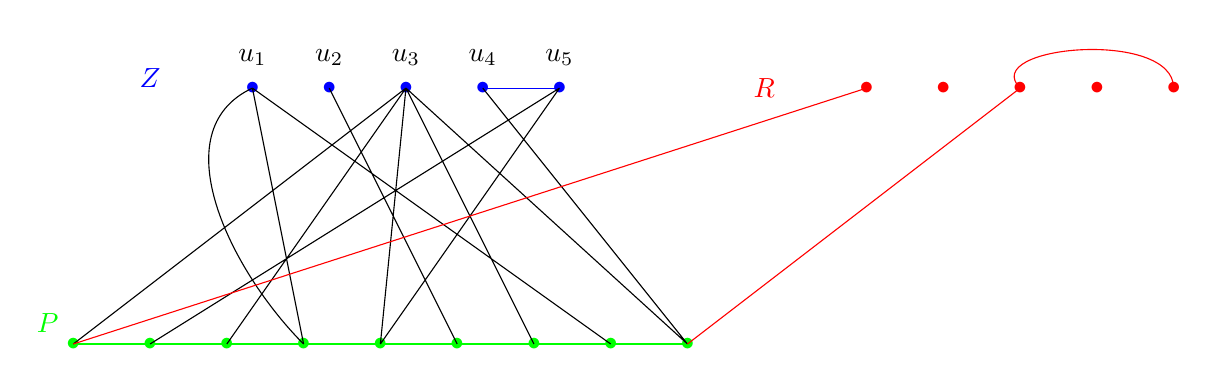
\begin{tikzpicture}[rotate=90, scale=1.3]


\node [green] (a) at (0.2,7) {$P$};
\node [green] (a) at (0,0.75) {$\bullet$};
\node [green] (a) at (0,1.5) {$\bullet$};
\node [green] (a) at (0,2.25) {$\bullet$};
\node [green] (a) at (0,3) {$\bullet$};
\node [green] (a) at (0,3.75) {$\bullet$};
\node [green] (a) at (0,4.5) {$\bullet$};
\node [green] (a) at (0,5.25) {$\bullet$};
\node [green] (a) at (0,6) {$\bullet$};
\node [green] (a) at (0,6.75) {$\bullet$};



\node [blue] (a) at (2.6,6) {$Z$};
\node [blue] (a1) at (2.5,2) {$\bullet$};
\node [blue] (a2) at (2.5,2.75) {$\bullet$};
\node [blue] (a) at (2.5,3.5) {$\bullet$};
\node [blue] (a) at (2.5,4.25) {$\bullet$};
\node [blue] (a) at (2.5,5) {$\bullet$};


\node [] (a) at (2.8,2) {$u_5$};
\node [] (a) at (2.8,2.75) {$u_4$};
\node [] (a) at (2.8,3.5) {$u_3$};
\node [] (a) at (2.8,4.25) {$u_2$};
\node [] (a) at (2.8,5) {$u_1$};

\draw[blue] (2.5,2)--(2.5,2.75);


 \draw[green] (0,0.75)-- (0,1.5) --(0,2.25) --
(0,3) --
 (0,3.75)-- 
 (0,4.5)-- 
 (0,5.25)--(0,6) --(0,6.75); 

 \draw[black]
(0,0.75)--(2.5,2.75)
(0,0.75)--(2.5,3.5) 
(0,1.5) --(2.5,5)
(0,2.25) --(2.5,3.5)
(0,3) --(2.5,4.25)
 (0,3.75)-- (2.5,2)
 (0,4.5)-- (2.5,5)
 (0,5.25)--(2.5,3.5)
(0,6) --(2.5,2)
(0,6.75)-- (2.5,3.5)
(0,3.75)--(2.5,3.5)
; 

\draw(0,4.5) to[out=45,in=115] (2.5,5);

\node [red] (a) at (2.5,-4) {$\bullet$};
\node [red] (a) at (2.5,-3.25) {$\bullet$};
\node [red] (a) at (2.5,-2.5) {$\bullet$};
\node [red] (a) at (2.5,-1.75) {$\bullet$};
\node [red] (a) at (2.5,-1) {$\bullet$};
\node [red] (a) at (2.5,0) {$R$};

\draw[red] (2.5,-2.5)--(0,0.75);
\draw[red] (2.5,-1)--(0,6.75);

\draw[red] (2.5,-4) to[out=0,in=45] (2.5,-2.5);


\end{tikzpicture}

\caption{An example of a path $P$ in $\cP$, $Z$ and $R$}
\label{figure_CP_paths}
\end{figure}


 
Observe that Lemma~\ref{lem:CP_path_creation} decomposes the graph into $k^{\OO(1)}$ simple structures, namely, paths in $\cal P$  combined together with a set of size $k^{\OO(1)}$. Note that the only {\em unbounded} objects in $G'$ are the paths in $\cal P$. The reason we can not reduce the size of $P$ is that a vertex in $Z$ can have unbounded neighbors on it. See Figure~\ref{figure_CP_paths} for an illustration. However,  
Lemma~\ref{lem:CP_path_creation} still  provides us the required decomposition which will be used to cast several instances of 
\shortULI{$\epsilon$}. In particular for every path $P \in \cal P$, we will have one instance of 
\shortULI{$\epsilon$}. We will compute \shortuli{$\epsilon$} for each of these instances and reduce the path size to get the desired kernel. 





\begin{theorem}
\label{thm:CPapprx}
For any $\epsilon>0$, there is polynomial sized $(1-\epsilon)$-approximate kernel for \CP. That is, \CP{} admits a PSAKS. 
\end{theorem}
\begin{proof}
Let $(G,k)$ be an input instance of \CP.  
The reduction algorithm ${\cal R}$ works as follows. It first runs the algorithm ${\cal A}$ mentioned in Lemma~\ref{lem:CP_path_creation}. If the algorithm returns $k$ vertex disjoint cycles, then ${\cal R}$ return these cycles. Otherwise, let $G'$, $Z$ and $R$ be the output of ${\cal A}$, satisfying four properties mentioned in Lemma~\ref{lem:CP_path_creation}. Important properties that will be most useful in our context are: 


\begin{itemize}
\setlength{\itemsep}{-2pt}
\item $\vert Z \vert \leq OPT(G,k)$, $\vert R\vert = \OO(k^4\log^4 k)$; and 
\item  $G'-(Z\cup R)$ is a collection $\cP$ of non trivial  
paths such that for any path $P\in \cP$ we have that no internal vertex of $P$ is adjacent to  
any vertex of $R$.
\end{itemize}
\noindent 
Now ${\cal R}$ will solve several instances of  \shortULI{$\epsilon$} to bound the length of each path in 
$\cP$. Towards this we fix a path $$P=v_1v_2\ldots v_{\ell}  \mbox{ in }  
\cP.$$ 
Our objective is to apply Lemma~\ref{lem:uni_lab_is} 
to reduce the length of $P$. 
Our algorithm finds a set of small number of relevant vertices on $P$ 
and reduces $P$ in {\em a single step} even though 
we use Lemma~\ref{lem:uni_lab_is} several times to identify relevant vertices.  Next we give the  construction for applying Lemma~\ref{lem:uni_lab_is} in order to find the relevant vertices. To find relevant vertices of $P$, we create $(\vert Z \vert +1)^2$ labelled interval graphs, one for every 
$(x,y)\in Z\cup \{\clubsuit\} \times Z \cup \{\clubsuit\}$  
with $Z\times Z$ being the set of labels. That is, for  the path $P$ and $(x,y)\in Z\cup \{\clubsuit\} \times Z \cup \{\clubsuit\}$ we create a  labelled interval graph $H_P^{(x,y)}$ as follows. Our labelling function will be denoted by  $\Gamma_P^{(x,y)}$.

\begin{enumerate}
\setlength{\itemsep}{-2pt}
\item The set of labels is $\Sigma=Z \times Z$. 
\item Let $P^{(x,y)}= v_r\ldots v_{r'}$ be the subpath of $P$ such that $v_{r-1}$ is the first vertex in $P$ adjacent to $x$ and $v_{r'+1}$ is the last vertex on $P$ adjacent to $y$.  If $x=\clubsuit$, then $v_r=v_1$ and if $y=\clubsuit$, then $v_{r'}=v_\ell$. Indeed, if $x=\clubsuit$ and $y=\clubsuit$ then $v_r=v_1$ and $v_{r'}=v_\ell$. 
\item We say that a subpath $Q'$ of $P^{(x,y)}$ is a {\em potential $(u_1,u_2)$-subpath}, 
where $(u_1,u_2)\in Z \times Z$, if   
either $u_1Q'u_2$ or $u_2Q'u_1$ is an induced path (induced cycle when $u_1=u_2$) in $G'$. Essentially, the potential subpath is trying to capture the way a cycle can interact with a subpath in $P$ with its neighbors on the cycle being $u_1$ and $u_2$.
\item For each $(u_1,u_2)\in Z \times Z$ 
and a potential $(u_1,u_2)$-subpath $Q'=v_i\ldots v_j$ we create an interval  
$I_{Q'}^{(u_1,u_2)}=[i,j]$ and  label it with $(u_1,u_2)$. That is, $\Gamma_P^{(x,y)}(I_{Q'}^{(u_1,u_2)})=(u_1,u_2)$. 
We would {\em like to emphasize} that when $u_1=u_2$ and $v_i=v_j$, we create an interval $I_{Q'}^{(u_1,u_2)}=[i,j]$ only if 
there are two edges between $u_1$ and $v_i$.  
Also notice that if we have created an interval $I_{Q'}^{(u_1,u_2)}=[i,j]$ with label $(u_1,u_2)$, then we have created an interval $I_{Q'}^{(u_2,u_1)}=[i,j]$ with label $(u_2,u_1)$ as well.  
\end{enumerate}

\begin{figure}

\centering

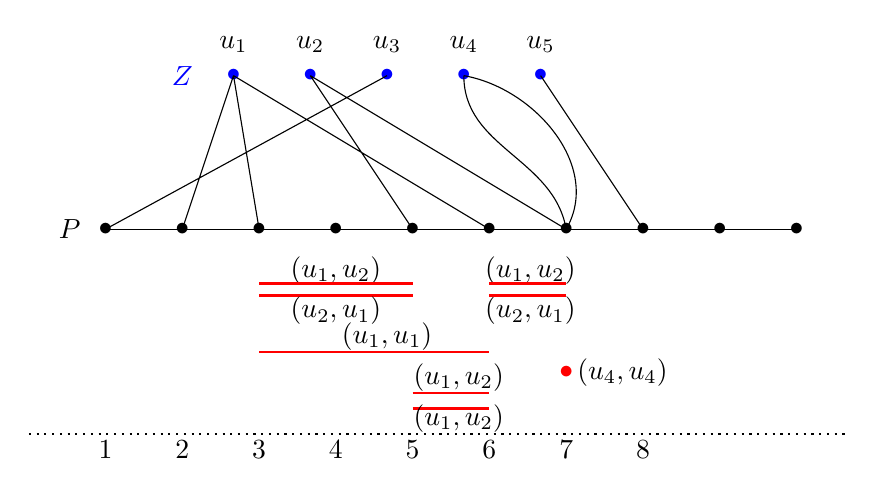
\begin{tikzpicture}[ scale=1.3]


\node [] (a) at (0.4,0) {$P$};
\node [] (a) at (0.75,0) {$\bullet$};
\node [] (a) at (1.5,0) {$\bullet$};
\node [] (a) at (2.25,0) {$\bullet$};
\node [] (a) at (3,0) {$\bullet$};
\node [] (a) at (3.75,0) {$\bullet$};
\node [] (a) at (4.5,0) {$\bullet$};
\node [] (a) at (5.25,0) {$\bullet$};
\node [] (a) at (6,0) {$\bullet$};
\node [] (a) at (6.75,0) {$\bullet$};
\node [] (a) at (7.5,0) {$\bullet$};



\node [blue] (a) at (1.5,1.5) {$Z$};
\node [blue] (a1) at (2,1.5) {$\bullet$};
\node [blue] (a2) at (2.75,1.5) {$\bullet$};
\node [blue] (a) at (3.5,1.5) {$\bullet$};
\node [blue] (a) at (4.25,1.5) {$\bullet$};
\node [blue] (a) at (5,1.5) {$\bullet$};


\node [] (a) at (2,1.8) {$u_1$};
\node [] (a) at (2.75,1.8) {$u_2$};
\node [] (a) at (3.5,1.8) {$u_3$};
\node [] (a) at (4.25,1.8) {$u_4$};
\node [] (a) at (5,1.8) {$u_5$};




 \draw[] (0.75,0)-- (1.5,0) --(2.25,0) --
(3,0) --
 (3.75,0)-- 
 (4.5,0)-- 
 (5.25,0)--(6,0) --(6.75,0)--(7.5,0); 

 \draw[black]
(2,1.5) -- (1.5,0)
(5,1.5)-- (6,0)
(2,1.5) -- (2.25,0)
(2,1.5) -- (4.5,0)
(2.75,1.5)-- (3.75,0)
(2.75,1.5)-- (5.25,0)
(4.25,1.5)to[out=-10,in=60](5.25,0)
(4.25,1.5)to[out=-90,in=100](5.25,0)
(3.5,1.5)--(0.75,0)
; 



\node [] (a) at (3,-0.4) {$(u_1,u_2)$};
\draw[line width=0.35mm,red] (2.25,-0.53)--(3.75,-0.53); 
\node [] (a) at (4.9,-0.4) {$(u_1,u_2)$};
\draw[line width=0.35mm,red] (2.25,-0.65)--(3.75,-0.65);
\node [] (a) at (3,-0.8) {$(u_2,u_1)$};
\node [] (a) at (4.9,-0.8) {$(u_2,u_1)$};
\draw[line width=0.35mm,red] (4.5,-0.53)-- (5.25,-0.53);
\draw[line width=0.35mm,red] (4.5,-0.65)-- (5.25,-0.65);
\node [] (a) at (5.8,-1.4) {$(u_4,u_4)$};
\node [red] (a) at (5.25,-1.4) {$\bullet$};


\draw[line width=0.35mm,red] (2.25,-1.2)--(4.5,-1.2);
\node [] (a) at (3.5,-1.05) {$(u_1,u_1)$};

\node [] (a) at (4.2,-1.45) {$(u_1,u_2)$};
\draw[line width=0.35mm,red] (3.75,-1.6)--(4.5,-1.6);
\draw[line width=0.35mm,red] (3.75,-1.75)--(4.5,-1.75);
\node [] (a) at (4.2,-1.85) {$(u_1,u_2)$};

\draw[thick, dotted] (0,-2)--(8,-2);
\node [] (a) at (.75,-2.15) {$1$};
\node [] (a) at (1.5,-2.15) {$2$};
\node [] (a) at (2.25,-2.15) {$3$};
\node [] (a) at (3,-2.15) {$4$};
\node [] (a) at (3.75,-2.15) {$5$};
\node [] (a) at (4.5,-2.15) {$6$};
\node [] (a) at (5.25,-2.15) {$7$};
\node [] (a) at (6,-2.15) {$8$};

\end{tikzpicture}

\caption{An example of $H_P^{(u_1,u_5)}$.  The interval representation of $H_P^{(u_1,u_5)}$ along with labels is drawn below 
the path $P$. The real line is represented using a dotted line.}
\label{figure_HP}
\end{figure}



This completes the construction of  $H_P^{(x,y)}$   and the labelling function
 $\Gamma_P^{(x,y)}$.  
See Figure~\ref{figure_HP} for an illustration.  
The fact that $H_P^{(x,y)}$  is an interval graph follows from the fact that in fact to construct  $H_P^{(x,y)}$, we have given an interval representation for it. 
Having, created the interval graph and a labelling function $\cal R$ runs the following steps. 



\begin{enumerate}
\setlength{\itemsep}{-2pt}
\item Now using Lemma~\ref{lem:CP_path_creation},  ${\cal R}$ computes 
a set $X^{(x,y)}_P$ such that $X^{(x,y)}_P$ is a \shortuli{$\frac{\epsilon}{2}$} of $H^{(x,y)}_P$. 
Now we define a few sets. 
\begin{eqnarray*}
S^{(x,y)}_P & = & \{v_i : i \mbox{ is an endpoint of an interval in } H^{(x,y)}_P \}\\
K_P& = & \{v_1,v_{\ell}\} \cup \bigcup_{u\in Z} \{ v : v \mbox{ is the first or last vertex on $P$ such that } uv\in E(G')\}\\ 
 S_P& = & \bigcup_{(x,y)\in  Z\cup \{\clubsuit\} \times Z \cup \{\clubsuit\}} S^{(x,y)}_P \\
 D_P & = & V(P)\setminus (S_P\cup K_P).
\end{eqnarray*}



\item Now, ${\cal R}$ will do the following modification to  shorten $P$: delete all the edges between 
$D_P$ and $Z$, and then contract all the remaining edges incident with vertices in $D_P$. In other words, let $\{v_{i_1},\ldots v_{i_{\ell'}}\}=S_P\cup K_P$, where $1=i_1<i_2<\ldots <i_{\ell'}=\ell$. Then delete $D_P$ and add edges $v_{i_j}v_{i_{j+1}}, j\in [\ell'-1]$. 
Let $P'$ be the path obtained from $P$, by the above process. We use the same vertex names in $P'$ as well to represent a
vertex. That is, if a vertex $u$ in $V(P)$ is not deleted to obtain $P'$, we use $u$ to represent the same vertex. 
\item Let $G''$ be the graph obtained after this modification has been done for all paths $P\in \cP$. 
Finally,  ${\cal R}$ returns $(G'',k)$ as the reduced instance. 
\end{enumerate}
\paragraph{Solution Lifting Algorithm.} 
Notice that $G''$ is a minor of $G'$ and hence a minor of $G$.  Given a set $S'$ of vertex disjoint cycles in 
$G''$, the solution lifting algorithm computes a set $S$ of vertex disjoint cycles in $G$ of cardinality 
$\vert S'\vert$ by doing reverse of the minor operations used to obtain $G''$ from $G$. All this can be done in polynomial time because  the solution lifting algorithm knows the 
minor operations done to get $G''$ from $G$.    

Next we need to prove the correctness of the algorithm. Towards that we first bound the size of $G''$.  

\medskip
\noindent 
{\bf Bounding the size of $G''$.} As a first step to bound the size of $G''$, we bound the chromatic number of $H_P^{(x,y)}$, where $P\in \cP$ and 
$(x,y)\in Z\cup \{\clubsuit\} \times Z \cup \{\clubsuit\}$. In fact what we will bound is the size of the maximum clique of $H_P^{(x,y)}$. 
\begin{claim}
\label{claim:CPpw}
For any $P\in \cP$ and $(x,y)\in Z\cup \{\clubsuit\} \times Z \cup \{\clubsuit\}$, $\chi(H_P^{(x,y)})=\OO(k^2)$. 
\end{claim}
\begin{proof}
To prove the claim, it is enough to show that the size of a maximum clique in $H_P^{(x,y)}$ is at most $\OO(k^2)$. 
Let $P^{(x,y)}= v_r\ldots v_{r'}$. We know that in the interval representation of $H_P^{(x,y)}$,  
all the intervals are contained in $[r,r']$. We claim that for any point $p\in [r,r']$ and $(u_1,u_2)\in Z \times Z$,  
the number of intervals labelled $(u_1,u_2)$ and containing the point $p$ is at most $2$. Towards a contradiction assume that there are 
three intervals $I_1=[i_1,j_1],I_2=[i_2,j_2],I_3=[i_3,j_3]$ such that $\Gamma_P^{(x,y)}(I_1)=\Gamma_P^{(x,y)}(I_2)=\Gamma_P^{(x,y)}(I_3)=(u_1,u_2)$ and all the 
intervals $I_1$, $I_2$ and $I_3$ contain the point $p$. Since for each $r\leq i,j\leq r'$ and $(u_1,u_2)\in Z\times Z$ 
we have created at most one interval $[i,j]$ with label $(u_1,u_2)$, all the intervals $I_1,I_2$ and $I_3$ are distinct intervals in the real line. 

We first claim that no interval in $\{I_1,I_2,I_3\}$ is same as $[p,p]$. Suppose $I_3=[p,p]$. 
Since all the interval in $\{I_1,I_2,I_3\}$, are different and $I_3=[p,p]$ we have that 
$I_1\neq [p,p]$, but contains $p$. This implies that either $i_1\neq p$ or $j_1\neq p$. We consider 
the case $i_1\neq p$. The case that $j_1\neq p$  is symmetric. 
Let $Q_1=v_{i_1}v_{i_1+1}\ldots v_{j_1}$. 
We know that $u_1v_pu_2$ is an induced 
path (induced cycle when $u_1=u_2$ and two edges between $u_1$ and $p$). This 
implies that neither $u_1Q_1u_2$ nor $u_2Q_1u_1$ is an induced path, 
because $v_p\in \{v_{i_1+1}\ldots v_{j_1}\}$. We would like to clarify that  
when ${j_1}=p$ and $u_1=u_2$, $u_1Q_1u_1$ is cycle 
and there are two edges between $v_{j_1}$ and $u_1$. 
This implies that $u_1Q_1u_1$ is a not an induced cycle.
 See Figure~\ref{figure_pointinterval} for illustration.  



\begin{figure}
\begin{subfigure}[b]{0.5\textwidth}
        \centering

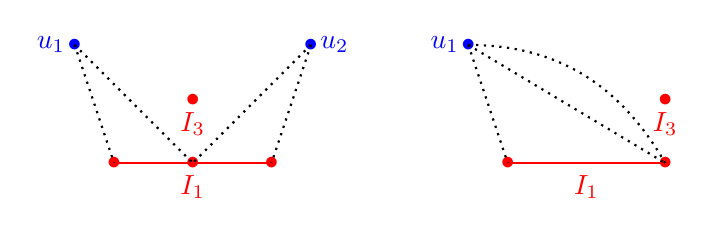
\begin{tikzpicture}[ scale=1]

\node[blue] at (-0.8,1.5) {$u_1$};
\node [blue] (a) at (-0.5,1.5) {$\bullet$};
\node [blue] (a) at (2.5,1.5) {$\bullet$};
\node[blue] at (2.8,1.5) {$u_2$};

\draw[line width=0.35mm,red] (0,0)--(2,0);
\node [red] (a) at (0,0) {$\bullet$};
\node [red] (a) at (2,0) {$\bullet$};
\node [red] (a) at (1,0.8) {$\bullet$};
\node [red] (a) at (1,0.5) {$I_3$};
\node [red] (a) at (1,-0.3) {$I_1$};
\node [red] (a) at (1,0) {$\bullet$};

\draw[thick, dotted] (-0.5,1.5) -- (0,0);
\draw[thick, dotted] (-0.5,1.5) -- (1,0);
\draw[thick, dotted] (2.5,1.5) -- (2,0);
\draw[thick, dotted] (2.5,1.5) -- (1,0);




\node[blue] at (4.2,1.5) {$u_1$};
\node [blue] (a) at (4.5,1.5) {$\bullet$};


\draw[line width=0.35mm,red] (5,0)--(7,0);
\node [red] (a) at (5,0) {$\bullet$};
\node [red] (a) at (7,0) {$\bullet$};
\node [red] (a) at (7,0.8) {$\bullet$};
\node [red] (a) at (7,0.5) {$I_3$};
\node [red] (a) at (6,-0.3) {$I_1$};
\draw[thick, dotted] (4.5,1.5) -- (5,0);
\draw[thick, dotted] (4.5,1.5) -- (7,0);
\draw[thick, dotted] (4.5,1.5)  to[out=0,in=120] (7,0);
\end{tikzpicture}
\end{subfigure}
\begin{subfigure}[b]{0.5\textwidth}
        \centering

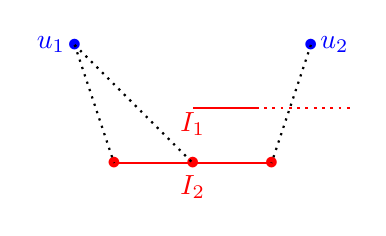
\begin{tikzpicture}[ scale=1]

\node[blue] at (-0.8,1.5) {$u_1$};
\node [blue] (a) at (-0.5,1.5) {$\bullet$};
\node [blue] (a) at (2.5,1.5) {$\bullet$};
\node[blue] at (2.8,1.5) {$u_2$};

\draw[line width=0.35mm,red] (0,0)--(2,0);
\draw[line width=0.35mm,red] (1,0.7)--(1.8,0.7);
\draw[line width=0.35mm,red,dotted] (1.8,0.7)--(3,0.7);
\node [red] (a) at (0,0) {$\bullet$};
\node [red] (a) at (2,0) {$\bullet$};
\node [red] (a) at (1,0.5) {$I_1$};
\node [red] (a) at (1,-0.3) {$I_2$};
\node [red] (a) at (1,0) {$\bullet$};

\draw[thick, dotted] (-0.5,1.5) -- (0,0);
\draw[thick, dotted] (-0.5,1.5) -- (1,0);
\draw[thick, dotted] (2.5,1.5) -- (2,0);



\end{tikzpicture}
\end{subfigure}
\caption{Illustration of 
proof of Claim~\ref{claim:CPpw}. The case when $I_3=[p,p]$ is drawn in the left and middle figures. 
The figure in the middle represents the 
case when $j_1=p$ and $u_1=u_2$.
The case when $I_1$ and $I_2$ intersects at strictly more than one point can be seen in the  right most figure.  
The black dotted curves represent the edges in the graph. }
\label{figure_pointinterval}
\end{figure}







Since $p$ is a common point in $I_1$, $I_2$ and $I_3$ and none of these intervals is equal to $[p,p]$, there are two intervals in 
$\{I_1,I_2,I_3\}$ such that they intersect at strictly more than one point. 
Without loss of generality we assume that the intersection of  $I_1$ and $I_2$
contains at least $2$ points. Also, since $I_1$ and $I_2$ are different intervals 
on the real line, one endpoint of an interval is fully inside another interval (not as the endpoint of the other interval). Let $Q_2=v_{i_2}v_{i_2+1}\ldots v_{j_2}$. 
Assume that $i_1\in (i_2,j_2)$. All other cases are symmetric to this case.  
We know that  $u_1v_{i_1}\in E(G')$ or $u_2v_{i_1}\in E(G')$.
This implies that 
neither $u_1Q_2u_2$ nor $u_2Q_2u_1$ is an induced path. This contradicts the fact that we created an interval 
$[i_2,j_2]$ with label $(u_1,u_2)$. See Figure~\ref{figure_pointinterval} for illustration.  


We have proved that for any point $p\in [r,r']$, the number of intervals containing   $p$ with the same label is upper bounded by  $2$. This implies that the cardinality of a largest clique in $H_P^{(x,y)}$ is at most twice the number of labels. Thus, the size of the largest cliques is upper bounded by $\OO(|Z|^2)$. 
By  Lemma~\ref{lem:CP_path_creation}, we know that $\vert Z \vert \leq OPT(G,k) \leq k+1$ and thus 
$\OO(|Z|^2)$ is bounded by $\OO(k^2)$. Since the chromatic number of an interval graph is upper bounded by the size of a maximum clique, the proof of the claim follows.  
\end{proof}




By 
Lemma~\ref{lem:CP_path_creation}, we know that 
$\vert \cP \vert= \OO(k^4\log^4 k)$. 
For each $P\in {\cal P}$ and $(x,y)\in Z\cup \{\clubsuit\} \times Z \cup \{\clubsuit\}$, we created a subset 
$S^{(x,y)}_P$ of $V(P)$ of cardinality $(|Z|^2 \cdot \chi(H_P^{(x,y)}) ^{\OO(\frac{2}{\epsilon}\log \frac{2}{\epsilon})}=k^{\OO(\frac{1}{\epsilon}\log \frac{1}{\epsilon})}$. Hence, the cardinality of $S_P$ is also upper bounded by $k^{\OO(\frac{1}{\epsilon}\log \frac{1}{\epsilon})}$. 
The cardinality of  $K_P$ is 
at most $2|Z|+2=\OO(k)$. 
This implies that the reduced path $P'$ has at most $k^{\OO(\frac{1}{\epsilon}\log \frac{1}{\epsilon})}$ vertices. 
Also, we know that $\vert \cP\vert =\OO(k^4\log^4 k)$, hence the total number of vertices across all the paths of $\cP$ after the reduction is upper bounded by $k^{\OO(\frac{1}{\epsilon}\log \frac{1}{\epsilon})}$. 
This together with the fact that $\vert Z \vert \leq OPT(G,k)$ and  $\vert R\vert = \OO(k^4\log^4 k)$ imply that  $\vert V(G'')\vert$ is upper bounded by $k^{\OO(\frac{1}{\epsilon}\log \frac{1}{\epsilon})}$. This completes the proof of upper bound on the size of $G''$. 


\medskip
\noindent 
{\bf Correctness of lossy reduction.} Finally, we show that indeed $(G'',k)$ is a  
$(1-\epsilon)$-approximate kernel for \CP. Towards this we show the following claim. 

\begin{claim}
\label{claim:optCP}
$OPT(G'',k)\geq (1-\epsilon)OPT(G',k)$. 
\end{claim}
\begin{proof}
Let $\CC$ be an optimum solution to $(G',k)$. Without loss of generality we can assume that 
each cycle in $\CC$ is a {\em chordless cycle}.  
Let $\cQ$ be the non-empty subpaths of cycles in $\CC$ induced in the graph $G'-(Z\cup R)$. 
That is, $\cQ$ is the collection of supaths in the intersection of $\CC$ and $\cP$.
For any $Q\in \cQ$, 
there exists two vertices $u,v\in R \cup Z$ such that $uQv$ is a subpath in $\CC$.
Because of property $(iv)$ of Lemma~\ref{lem:CP_path_creation}, for any $Q\in \cQ$ with $\vert V(Q)\vert =1$, at least one of the endpoint of $Q$ is connected to a vertex from $Z$ in the cycle packing $\CC$. 
We say a path $Q'$ is a {\em substitute} for $Q\in \cQ$ if $uQ'v$ is a subpath in $G''$ where 
$u,v\in R\cup Z$ and $uQv$ is a subpath in $\CC$. 
In what follows,   for at least $(1-\epsilon)\vert \cQ\vert$ paths in $\cQ$, we identify substitutes in 
the reduced graph $G''$ which are pairwise vertex disjoint.




We partition the paths in $\cQ$ into $\cQ_1$ and $\cQ_2$. 
Notice that $Q_i\in \cQ$ is a subpath of a cycle $C\in \CC$ and the neighbors (could be the same) 
of  both the endpoints  of $Q_i$ on $C$ are in 
$R\cup Z$. If the neighbors of both endpoints of $Q_i$  on $C$ are in $Z$, then we include $Q_i$ in $\cQ_1$.  Otherwise $Q_i$ is in $\cQ_2$. 
See Figure~\ref{figure_cyclepathintersection} for an illustration. 
For each $Q\in \cQ_2$, we give a substitute path 
as follows. 
We know that there is a path $P\in\cP$ such that  either $P=QQ'$ or $P=Q'Q$ for some $Q'$ where $V(Q')$ can be 
an empty set too.
If $Q=P$, then we replace $Q$ with $P'$ 
(Note that $P'$ is the path obtained from $P$ in the reduction process). Also, notice that end vertices of $P$ and $P'$ are same 
(because endvertices of $P$ belong to $K_P$) 
and hence $P'$ is a substitute for 
$Q$. Suppose $P=QQ'$ where $V(Q')\neq \emptyset$. Let $C_Q$ be the cycle in $\CC$ such that $Q$ is a subpath of $C_Q$. 
Let $Q=v_1\ldots v_{d}$. Let $z$ be the neighbour of $v_d$ in $C_Q$ which is from $Z$ (recall that 
 no internal vertex of $P$ is adjacent to  any vertex of $R$).  
Since 
$C_Q$ is a chordless cycle, none of $v_1,\ldots, v_{d-1}$ is adjacent to $z$. This implies that  $v_1,v_{d}\in K_P$ and hence 
$P'$ contains a subpath $P'_{Q}$ from $v_1$ to $v_{d-1}$ with internal vertices from $\{v_2,\ldots,v_{d-1}\}$. In this case 
$P'_{Q}$ is a substitute for $Q$. In a similar way, we can construct a substitute for $Q$ when  $P=Q'Q$ where $V(Q')\neq \emptyset$. 
Let $\cQ'_2$ be the set of substitute paths constructed for paths in $\cQ_2$. Notice that $\cQ'_2$ 
is a collection of vertex disjoint paths in $G''-(Z\cup R)$ and it has one substitute path for each $Q\in \cQ_2$. 
See Figure~\ref{figure_cyclepathintersection} for an illustration. 




\begin{figure}

\begin{subfigure}[b]{0.5\textwidth}
        \centering
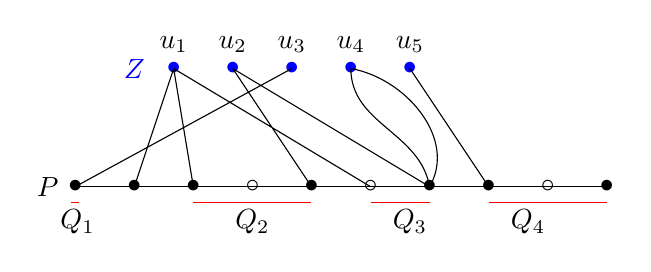
\begin{tikzpicture}[ scale=1]


\node [] (a) at (0.4,0) {$P$};
\node [] (a) at (0.75,0) {$\bullet$};
\node [] (a) at (1.5,0) {$\bullet$};
\node [] (a) at (2.25,0) {$\bullet$};
\node [] (a) at (3,0) {$\circ$};
\node [] (a) at (3.75,0) {$\bullet$};
\node [] (a) at (4.5,0) {$\circ$};
\node [] (a) at (5.25,0) {$\bullet$};
\node [] (a) at (6,0) {$\bullet$};
\node [] (a) at (6.75,0) {$\circ$};
\node [] (a) at (7.5,0) {$\bullet$};

\node [blue] (a) at (1.5,1.5) {$Z$};
\node [blue] (a1) at (2,1.5) {$\bullet$};
\node [blue] (a2) at (2.75,1.5) {$\bullet$};
\node [blue] (a) at (3.5,1.5) {$\bullet$};
\node [blue] (a) at (4.25,1.5) {$\bullet$};
\node [blue] (a) at (5,1.5) {$\bullet$};


\node [] (a) at (2,1.8) {$u_1$};
\node [] (a) at (2.75,1.8) {$u_2$};
\node [] (a) at (3.5,1.8) {$u_3$};
\node [] (a) at (4.25,1.8) {$u_4$};
\node [] (a) at (5,1.8) {$u_5$};



 \draw[] (0.75,0)-- (1.5,0) --(2.25,0) --
(3,0) --
 (3.75,0)-- 
 (4.5,0)-- 
 (5.25,0)--(6,0) --(6.75,0)--(7.5,0); 

 \draw[black]
(2,1.5) -- (1.5,0)
(5,1.5)-- (6,0)
(2,1.5) -- (2.25,0)
(2,1.5) -- (4.5,0)
(2.75,1.5)-- (3.75,0)
(2.75,1.5)-- (5.25,0)
(4.25,1.5)to[out=-10,in=60](5.25,0)
(4.25,1.5)to[out=-90,in=100](5.25,0)
(3.5,1.5)--(0.75,0)
; 


 \draw[red] (0.7,-0.2)-- (0.8,-0.2) 
(2.25,-0.2) --(3.75,-0.2) 
 (4.5,-0.2)--(5.25,-0.2)
(6,-0.2) --(6.75,-0.2)--(7.5,-0.2); 

\node [] (a) at (0.78,-0.45) {$Q_1$};
\node [] (a) at (3,-0.45) {$Q_2$};
\node [] (a) at (5,-0.45) {$Q_3$};
\node [] (a) at (6.5,-0.45) {$Q_4$};
\end{tikzpicture}
\end{subfigure}
\begin{subfigure}[b]{0.5\textwidth}
        \centering
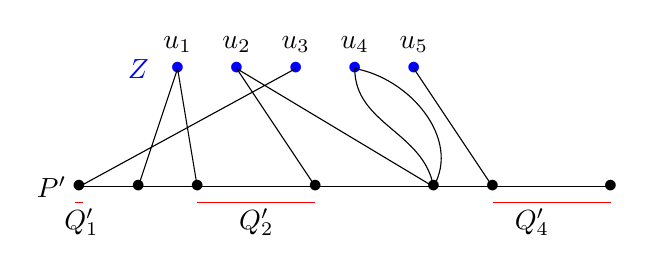
\begin{tikzpicture}[ scale=1]


\node [] (a) at (0.4,0) {$P'$};
\node [] (a) at (0.75,0) {$\bullet$};
\node [] (a) at (1.5,0) {$\bullet$};
\node [] (a) at (2.25,0) {$\bullet$};
\node [] (a) at (3.75,0) {$\bullet$};
\node [] (a) at (5.25,0) {$\bullet$};
\node [] (a) at (6,0) {$\bullet$};
\node [] (a) at (7.5,0) {$\bullet$};

\node [blue] (a) at (1.5,1.5) {$Z$};
\node [blue] (a1) at (2,1.5) {$\bullet$};
\node [blue] (a2) at (2.75,1.5) {$\bullet$};
\node [blue] (a) at (3.5,1.5) {$\bullet$};
\node [blue] (a) at (4.25,1.5) {$\bullet$};
\node [blue] (a) at (5,1.5) {$\bullet$};


\node [] (a) at (2,1.8) {$u_1$};
\node [] (a) at (2.75,1.8) {$u_2$};
\node [] (a) at (3.5,1.8) {$u_3$};
\node [] (a) at (4.25,1.8) {$u_4$};
\node [] (a) at (5,1.8) {$u_5$};



 \draw[] (0.75,0)-- (1.5,0) --(2.25,0) --
(3,0) --
 (3.75,0)-- 
 (4.5,0)-- 
 (5.25,0)--(6,0) --(6.75,0)--(7.5,0); 

 \draw[black]
(2,1.5) -- (1.5,0)
(5,1.5)-- (6,0)
(2,1.5) -- (2.25,0)
(2.75,1.5)-- (3.75,0)
(2.75,1.5)-- (5.25,0)
(4.25,1.5)to[out=-10,in=60](5.25,0)
(4.25,1.5)to[out=-90,in=100](5.25,0)
(3.5,1.5)--(0.75,0)
; 


 \draw[red] (0.7,-0.2)-- (0.8,-0.2) 
(2.25,-0.2) --(3.75,-0.2) 
(6,-0.2) --(6.75,-0.2)--(7.5,-0.2); 

\node [] (a) at (0.78,-0.45) {$Q'_1$};
\node [] (a) at (3,-0.45) {$Q'_2$};
\node [] (a) at (6.5,-0.45) {$Q'_4$};
\end{tikzpicture}
\end{subfigure}




\caption{An example of intersection of $\CC$ and a path $P\in \PP$. 
The vertices in $P$ colored black belong to $V(P')$. 
The intersection of $\CC$ and $P$ are the set of paths 
$\QQ=\{Q_1,Q_2,Q_3,Q_4\}$. Here $Q_2,Q_3\in \QQ_1$ and $Q_1,Q_4\in \QQ_2$. 
The substitute paths for $\QQ$ is in the figure at the right hand side}
\label{figure_cyclepathintersection}
\end{figure}


































Now we construct substitute paths for $\cQ_1$. Here, we construct substitute paths for at least $(1-{\epsilon})\vert \cQ_1\vert$ 
paths and these paths will be vertex disjoint. Moreover, these paths will be vertex disjoint from the paths in $\cQ_2'$ as well. 
Let $P$ be a path in ${\cal P}$ such that at least one path in $\cQ_1$ is a subpath of $P$. 
Let $\cQ_1(P)\subseteq \cQ_1$ be a subset of $\cQ_1$ containing all the paths in $\cQ_1$ that is a subpath of $P$. 
There are at most two paths in $\cQ_2$ which 
are subpaths of $P$. Let $F$ and $L$ be these paths, where $F$ and $L$ could be empty too. 
 Let the neighbours of $F$ and $L$ in $Z$ in the cycle packing $\CC$ be $x$ and $y$, respectively 
(here, $x=\clubsuit$ if $F=\emptyset$ and $y=\clubsuit$ if $L=\emptyset$).  
Then, consider the  following decomposition of path $P=FP^\star L$. We claim that $P^\star=P^{(x,y)}$. That is, $P^\star$ is a path for which we would have created the interval graph $H_P^{(x,y)}$.  
Observe that, if $F$ is non-empty then $x$  does not have any neighbor on $F$ as cycles in $\cal C$ are {\em chordless}. Similarly, if $L$ is non-empty then $y$ does not have any neighbor on $L$. 
Thus, if $F$ and $L$ are both non-empty then indeed the {\em last} vertex of $F$ is the {\em first}  vertex on $P$ that is a neighbor of $x$ and the {\em first} vertex of $L$ is the {\em last} vertex on $P$ that is a neighbor of $y$. This implies that indeed we would have created the interval graph $H_P^{(x,y)}$. We can argue similarly if either $F$ is empty or $L$ is empty.  
Now consider the interval graph $H_P^{(x,y)}$. This graph is constructed from $P^{(x,y)}$. 
Since 
each cycle in $\CC$ is a chordless cycle, we have that 
each subpath $Q\in \cQ_1(P)$ is a potential $(u_1,u_2)$-subpath of $P^{(x,y)}$ where 
either $u_1Qu_2$ or $u_2Qu_1$ is a subpath of $\CC$ and $u_1,u_2\in Z$.
Since each vertex in $V(\CC)$ has degree two in $\CC$, 
for a pair $(u_1,u_2)$ we have {\em at most two potential $(u_1,u_2)$ paths} 
$Q_1$ and $Q_2$ in $\cQ_1(P)$. Also note that these supaths $Q_1$ and $Q_2$ are 
potential $(u_2,u_1)$-subpaths as well. So when there are two paths $Q_1,Q_2\in \cQ_1(P)$ 
such that $u_1Q_1 u_2$ and $u_1 Q_2 u_2$ are subpaths of $\CC$, then we consider $Q_1$ 
as a potential $(u_1,u_2)$-subpath and $Q_2$ as  a potential $(u_2,u_1)$-subpath.  
Now we can consider $\cQ_1(P)$ as a set of potential subpaths of $P^{(x,y)}$. 
That is, for each 
$Q\in \cQ_1(P)$, there is an interval $I^{(u_1,u_2)}_Q$ with label $(u_1,u_2)$ 
and $(u_1,u_2)$ is not a label of any other intervals corresponding to a subpath in 
$\cQ_1(P)\setminus \{Q\}$.
Let ${\cal I}_1(P)$ be the set of interval created for the potential subpaths in $\cQ_1(P)$. 
We have explained that for 
any $(u_1,u_2)\in Z \times Z$, there is at most one potential $(u_1,u_2)$-subpath in $\cQ_1(P)$. 
Also notice that, since $\cQ_1(P)$ is a collection of vertex disjoint paths, the interval 
constructed for corresponding potential subpaths are disjoint. This 
implies that ${\cal I}_1(P)$ is an independent set in  $H_P^{(x,y)}$ and 
$\vert \Gamma_P^{(x,y)}({\cal I}_1(P))\vert= \vert {\cal I}_1(P)\vert$. 
By Lemma~\ref{lem:uni_lab_is}, we have that 
there is a subset $\Sigma'\subseteq \Gamma_P^{(x,y)}({\cal I}_1(P))$
such that there is an independent set $S$ of cardinality $(1-\frac{\epsilon}{2})\vert {\cal I}_1(P)\vert$
in $X_P^{(x,y)}$ and $\Gamma_P^{(x,y)}(S)=\Sigma'$. This implies that there are at least 
$(1-\frac{\epsilon}{2})\vert {\cal I}_1(P)\vert = (1-\frac{\epsilon}{2})\vert \cQ_1(P)\vert$ 
of paths in $\cQ_1(P)$ has {\em substitute paths} in $P'$ which are vertex disjoint from 
$F$ and $L$, where $P'$ is the path obtained from $P$ in the reduction process using Lemma~\ref{lem:uni_lab_is}. This implies that for 
each $P\in \cP$, at least $(1-\frac{\epsilon}{2})\vert \cQ_1(P)\vert$ paths has 
substitute paths in $G''$ and they are vertex disjoint subpaths of $P'$ and does not intersect 
with $F$ and $L$. We denote the set of substitute paths in $P'$ by $\cQ_1'(P')$. 
This implies that the substitute paths for $\cQ_1$ are vertex disjoint and they are vertex disjoint from the 
substitute paths for $\cQ_2$. Let these substitute paths form a set $\cQ_1'=\cup_{P\in \cP}\cQ_1'(P')$. 
Also notice that 
since each vertex $u\in Z$, has degree at most $2$ in $\CC$ and $\vert Z \vert\leq OPT(G',k)$, 
the total number of paths in $\cQ_1$ is at most $2OPT(G',k)$.
From each $\cQ_1(P)$, at least $(1-\frac{\epsilon}{2})\vert \cQ_1(P)\vert$ paths have 
substitute paths in $G''$. Recall that, 
\[ \cQ_1 =\biguplus_{P\in \cP}\cQ_1(P) \mbox{ and }  \cQ_1' =\biguplus_{P\in \cP}\cQ_1'(P').\]
That is, $\cQ_1$ ($\cQ_1'$) is the disjoint union of $\cQ_1(P)$ ($\cQ_1'(P')$) for $P\in \cP$. Thus, 
\begin{eqnarray*}
\vert \cQ_1\vert -  \vert \cQ_1' \vert &= & \sum_{P\in \cP} \vert \cQ_1(P) \vert -  \vert \cQ_1'(P') \vert \\
& \leq & \sum_{P\in \cP} \vert \cQ_1(P) \vert - \left(1- \frac{\epsilon}{2}\right) \vert \cQ_1(P) \vert \\
& = & \left(\sum_{P\in \cP} \frac{\epsilon}{2} \vert \cQ_1(P) \vert  \right)=  \frac{\epsilon}{2} \vert \cQ_1 \vert.
\end{eqnarray*}
This implies that $\vert \cQ_1\vert-\vert \cQ_1'\vert \leq  \frac{\epsilon}{2} \vert \cQ_1 \vert \leq \epsilon OPT(G',k)$. This implies that  $\cQ_1'\cup \cQ_2'$ contains at least $(1-\epsilon)OPT(G',k)$ substitute paths. Each path in $\cQ$ for which we do not have a substitute path can destroy at most one cycle in 
$\CC$. Recall that, $\CC$  is an optimum solution to $(G',k)$. This implies that $G''$
contains at least $(1-\epsilon)OPT(G',k)$ vertex disjoin cycles. 
This completes the proof of the claim. 
\end{proof}
By Lemma~\ref{lem:CP_path_creation}, we know that $OPT(G',k)=OPT(G,k)$ and hence 
by Claim~\ref{claim:optCP} we get that $OPT(G'',k)\geq (1-\epsilon)OPT(G,k)$.   
We know that given a solution ${\cal S}'$ of $(G'',k)$ the solution lifting algorithm will output a solution ${\cal S}$ of same cardinality
for $(G,k)$. Therefore, we have  
$$\frac{\vert{\cal S}\vert}{OPT(G,k)}\geq (1-\epsilon) \frac{\vert{\cal S}'\vert}{OPT(G'',k)}.$$
This gives the desired PSAKS for \CP{} and completes the proof.
\end{proof}


